%%%%%%%%%%%%%%%%%%%%%%%%%%%%%%%%% author.tex %%%%%%%%%%%%%%%%%%%%%%%%%%%%%%%%%
%
% sample root file for your "contribution" to a contributed volume
%
% Use this file as a template for your own input.
%
%%%%%%%%%%%%%%%%%%%%%%%%%%%%%%%%%% Springer %%%%%%%%%%%%%%%%%%%%%%%%%%%%%%%%%%



% RECOMMENDED %%%%%%%%%%%%%%%%%%%%%%%%%%%%%%%%%%%%%%%%%%%%%%%%%%%%%%%%%%%%%%%%
\documentclass[graybox]{svmult}

% choose options for [] as required from the list
% in the Reference Guide

\usepackage{mathptmx}           % selects Times Roman as basic font
\usepackage{helvet}             % selects Helvetica as sans-serif font
\usepackage{courier}            % selects Courier as typewriter font
\usepackage{type1cm}            % activate if the above 3 fonts are
                                % not available on your system

%\usepackage{makeidx}            % allows index generation
%\usepackage[dvips]{graphicx}
%\usepackage[dvipdfmx]{graphicx}
\usepackage{graphicx}           % standard LaTeX graphics tool when including figure files

%\usepackage{subfig}
\usepackage{subfigure}
\usepackage{algorithmic}
\usepackage{algorithm}
\usepackage{cite}


%\usepackage{multicol}           % used for the two-column index
%\usepackage[bottom]{footmisc}   % places footnotes at page bottom
\usepackage{booktabs} 
\usepackage{arydshln}
%\usepackage{natbib}
%\usepackage[numbers]{natbib}
%\usepackage[round]{natbib}
%\usepackage[numbers,sort&compress]{natbib}
%\bibliographystyle{unsrtnat}
%\usepackage[numbers,sort&compress]{natbib}

\usepackage{newtxtext,newtxmath} %これで英文字も綺麗なベクターになる(timesより優秀)
\def\vector#1{\mbox{\boldmath $#1$}}



% see the list of further useful packages
% in the Reference Guide

\makeindex             % used for the subject index
                       % please use the style svind.ist with
                       % your makeindex program


%%%%%%%%%%%%%%%%%%%%%%%%%%%%%%%%%%%%%%%%%%%%%%%%%%%%%%%%%%%%%%%%%%%%%%%%%%%%%%

\begin{document}
\title*{Wearable Haptic Feedback Glove for Texture Rendering in Virtual Reality}

% Use \titlerunning{Short Title} for an abbreviated version of
% your contribution title if the original one is too long
\titlerunning{Glove for Texture Rendering in Virtual Reality}

\author{Korntawat Witchuvanit, Makio Ishihara}

% Use \authorrunning{Short Title} for an abbreviated version of
% your contribution title if the original one is too long
\authorrunning{K. Witchuvanit, M. Ishihara}

\institute{
	Korntawat Witchuvanit
	\at Graduate School of Engineering, Fukuoka Institute of Technology,\\
	3-30-1 Wajiro-Higashi, Higashi-Ku, Fukuoka 811-0295, Japan,\\ 
	\email{mfm23201@bene.fit.ac.jp}
	\and 
	Makio Ishihara 
	\at Department of Information and Communication Engineering, Fukuoka Institute of Technology,\\
	3-30-1 Wajiro-Higashi, Higashi-Ku, Fukuoka 811-0295, Japan,\\ 
	\email{m-ishihara@fit.ac.jp}
	}
% Use the package "url.sty" to avoid
% problems with special characters
% used in your e-mail or web address

\maketitle 

%%%%%%%%%%%%%%%%%%%%%%%%%%%%%%%%%%%%%%%%%%%%%%%%%%%%%%%%%%%%%%%%%%%%%%%%%
%%%%%%%%%%%%%%%%%%%%%%%%%%%%%%%%%%%%%%%%%%%%%%%%%%%%%%%%%%%%%%%%%%%%%%%%%
% Abstract
%%%%%%%%%%%%%%%%%%%%%%%%%%%%%%%%%%%%%%%%%%%%%%%%%%%%%%%%%%%%%%%%%%%%%%%%%
%%%%%%%%%%%%%%%%%%%%%%%%%%%%%%%%%%%%%%%%%%%%%%%%%%%%%%%%%%%%%%%%%%%%%%%%%

\abstract{
Virtual reality (VR) provides immersive experiences through multisensory feedback, enhancing user interaction with digital environments. One key immersion aspect is texture rendering, which is commonly achieved through visual and auditory cues. Incorporating haptic feedback for realistic texture perception is a mainstream of Human-Computer Interaction (HCI) research activities and it remains a challenge. Most existing methods rely on hand-held devices, often limiting natural hand movements. This research explores the development and performance of a wearable device equipped with flex sensors, a Motion Processing Unit (MPU), and a coin motor, enabling texture perception at three vibration granularities. The results show that participants can distinguish various textures based on their smoothness, particularly identifying differences between them.
}

%%%%%%%%%%%%%%%%%%%%%%%%%%%%%%%%%%%%%%%%%%%%%%%%%%%%%%%%%%%%%%%%%%%%%%%%%
%%%%%%%%%%%%%%%%%%%%%%%%%%%%%%%%%%%%%%%%%%%%%%%%%%%%%%%%%%%%%%%%%%%%%%%%%
% Introduction
%%%%%%%%%%%%%%%%%%%%%%%%%%%%%%%%%%%%%%%%%%%%%%%%%%%%%%%%%%%%%%%%%%%%%%%%%
%%%%%%%%%%%%%%%%%%%%%%%%%%%%%%%%%%%%%%%%%%%%%%%%%%%%%%%%%%%%%%%%%%%%%%%%%
\section{Introduction}
Virtual reality has evolved into a powerful tool for immersive experiences across diverse domains such as gaming, training, and therapy \cite{slater2016enhancing}. By integrating visual, auditory, and interactive components, VR environments offer users the sensation of presence, significantly enhancing engagement and realism \cite{biocca2013communication}. Advances in display technologies, motion tracking systems, and spatial audio have greatly improved immersion; however, realistic tactile perception remains a significant challenge, constraining overall sensory fidelity in VR applications.

Haptic feedback is essential in bridging this sensory gap, as it introduces tactile stimuli that simulate real-world touch sensations \cite{culbertson2018haptics}. Various haptic devices, including vibrotactile actuators, force-feedback systems, and wearable gloves, have been developed to enhance tactile realism. Although handheld controllers are commonly used, they often restrict natural hand movements, negatively affecting immersion. Wearable solutions offer a promising alternative by enabling direct and intuitive hand interactions with virtual objects \cite{pacchierotti2017wearable}. Nonetheless, designing lightweight, responsive, and versatile wearable haptic systems remains an open challenge within HCI research.

To address these limitations, we propose a custom wearable glove equipped with flex sensors, MPU, and a coin motor for providing nuanced haptic feedback. Our glove enhances virtual texture perception by modulating vibration frequencies across three distinct granularities, selected based on their demonstrated influence on perceived texture realism \cite{strohmeier2017generating,bensmaia2005vibrations}. This paper's contributions include the development of a lightweight and responsive wearable device and the empirical evaluation of users' tactile perception of texture granularity, thereby advancing the realism and immersion of VR haptic feedback systems.

%%%%%%%%%%%%%%%%%%%%%%%%%%%%%%%%%%%%%%%%%%%%%%%%%%%%%%%%%%%%%%%%%%%%%%%%%
%%%%%%%%%%%%%%%%%%%%%%%%%%%%%%%%%%%%%%%%%%%%%%%%%%%%%%%%%%%%%%%%%%%%%%%%%
% Related Work
%%%%%%%%%%%%%%%%%%%%%%%%%%%%%%%%%%%%%%%%%%%%%%%%%%%%%%%%%%%%%%%%%%%%%%%%%
%%%%%%%%%%%%%%%%%%%%%%%%%%%%%%%%%%%%%%%%%%%%%%%%%%%%%%%%%%%%%%%%%%%%%%%%%
\section{Related Work}\label{sec:nssdn}
Recent advancements in haptic feedback systems have emphasized simulating realistic texture granularity using techniques like Pulse Width Modulation (PWM) and advanced tactile technologies. Bach et al. \cite{bach2023enhanced} notably enhanced tactile experiences using Pb(Zr,Ti)O₃ thin films on German silver foils, contributing to more precise texture sensations in microsystem technologies. Otake et al. \cite{otake2022vibrotactile} explored combining vibrotactile and electrostatic-friction stimuli, significantly improving texture realism for touch-panel applications.

Machine learning approaches also gained prominence for generating realistic tactile feedback. Zhang et al. \cite{zhang2022texsensegan} developed TexSenseGAN, leveraging Generative Adversarial Networks (GANs) to optimize vibrotactile feedback based on user input, enhancing texture realism intuitively. Moreover, Strohmeier and Hornbæk \cite{strohmeier2017generating} examined how parameters like granularity, amplitude, and timbre affect perceived haptic textures, identifying granularity as particularly influential for users' perception of bumpiness and smoothness.

PWM technology, frequently integrated into these systems, provides dynamic adjustments of vibration intensity and frequency, enabling precise simulations of texture granularity. This capability facilitates generating tactile sensations ranging from smooth surfaces to coarse textures. However, despite significant progress, existing systems often fail to offer fully intuitive and unrestricted hand interactions due to physical constraints or limited responsiveness.

Our research addresses this gap by employing PWM for precise granularity simulation in wearable haptic devices, focusing explicitly on texture perception within virtual environments. By providing dynamic, responsive, and intuitive tactile feedback, our approach enhances user immersion and interaction realism in VR applications.


%%%%%%%%%%%%%%%%%%%%%%%%%%%%%%%%%%%%%%%%%%%%%%%%%%%%%%%%%%%%%%%%%%%%%%%%%
%%%%%%%%%%%%%%%%%%%%%%%%%%%%%%%%%%%%%%%%%%%%%%%%%%%%%%%%%%%%%%%%%%%%%%%%%
% Intra/Inter Slice Handover
%%%%%%%%%%%%%%%%%%%%%%%%%%%%%%%%%%%%%%%%%%%%%%%%%%%%%%%%%%%%%%%%%%%%%%%%%
%%%%%%%%%%%%%%%%%%%%%%%%%%%%%%%%%%%%%%%%%%%%%%%%%%%%%%%%%%%%%%%%%%%%%%%%%
\section{Intra/Inter-Slice Handover}\label{sec:shd}
The HO can be classified into two main types based on network and access technology: horizontal and vertical. The horizontal HO occurs within the same access technology, such as when a user moves between the BSs in a 5G network. This type of HO is commonly used in situations where the user remains within the same RAT, ensuring smooth transitions without changing the underlying technology. In contrast, the vertical HO involves transitioning between different RATs, such as when a mobile device switches from a cellular network to a Wireless Local Area Network (WLAN). Vertical HOs are critical for maintaining connectivity in heterogeneous networks, where multiple access technologies are available, and they enable devices to seamlessly shift between different network infrastructures while optimizing performance and resource usage~\cite{10147830, 8141874, PALMIERI2020107365}. 

Inter-slice HO is an important process that transfers a device's connection from one NS to another within the same physical network infrastructure. This process is vital for maintaining QoS and Quality of Experience (QoE) when a device's service requirements change due to user activity or mobility patterns~\cite{ren2021fast, sajjad2022inter}. Efficient inter-slice HO is essential to meet the demands of high real-time services, such as 5G-assisted drones and autonomous driving. This capability is essential for maintaining optimal service because the requirements of user context or service evolve. Some examples of inter-slice HO are presented in following. 
\begin{itemize}
\item \textbf{Different vertical industries with different operators:}  Transitioning between slices dedicated to different industries (e.g., healthcare to automotive) managed by different network operators. This type of handover is complex due to the need for interoperability across operators' networks, each with its own set of policies, security standards, and service level agreements (SLAs).  
\item \textbf{Different vertical industries with the same operators:} Handovers can occur between slices customized for different industries within a single network operator. This means that within a network, various slices, each optimized for specific industries or use cases, can seamlessly handover connections as users transition between different slices. For instance, moving a connection from a slice serving IoT devices in smart agriculture to another serving URLLC for autonomous vehicles.
\item \textbf{Same vertical industries with different operators:} Handovers between slices serving the same industry but controlled by different operators, such as in cross-border scenarios for connected vehicles or international smartphone roaming. It needs to ensure continuous service in applications where users or devices move across different operators' coverage areas but needs consistent QoS and features.
\end{itemize}






%%%%%%%%%%%%%%%%%%%%%%%%%%%%%%%%%%%%%%%%%%%%%%%%%%%%%%%%%%%%%%%%%%%%%%%%%
%%%%%%%%%%%%%%%%%%%%%%%%%%%%%%%%%%%%%%%%%%%%%%%%%%%%%%%%%%%%%%%%%%%%%%%%%
% Proposed Fuzzy-based System
%%%%%%%%%%%%%%%%%%%%%%%%%%%%%%%%%%%%%%%%%%%%%%%%%%%%%%%%%%%%%%%%%%%%%%%%%
%%%%%%%%%%%%%%%%%%%%%%%%%%%%%%%%%%%%%%%%%%%%%%%%%%%%%%%%%%%%%%%%%%%%%%%%%

\section{Proposed Fuzzy-based System}\label{sec:proposed}

In Fig.~\ref{fig:5GHO} is provided the overview of proposed system. Each evolved Base Station (eBS) operates under the control of SDN controller, which is responsible for issuing control commands that govern communication and data transmission between the eBS and User Equipment (UE). The SDN controller plays a pivotal role in orchestrating the network, ensuring dynamic resource allocation, and optimizing traffic flow in real time. The SDN controller acts as a centralized control unit, bridging communication between the eBS and the 5G core network. It coordinates with the core network elements, such as the Access and Mobility Management Function (AMF) and the User Plane Function (UPF), to ensure a seamless HO process and maintain uninterrupted connectivity and efficient resource management throughout the network.

Each eBS supports multiple NSs, where each slice is dedicated to specific types of applications or services, such as enhanced Mobile Broadband (eMBB), Ultra-Reliable Low-Latency Communication (URLLC), or Massive Machine Type Communication (mMTC). This slicing capability enables the network to deal with diverse requirements simultaneously, enhancing the flexibility and efficiency of the 5G infrastructure.

%5gsdn
%\vspace{1cm}
\begin{figure}[h]\centering
	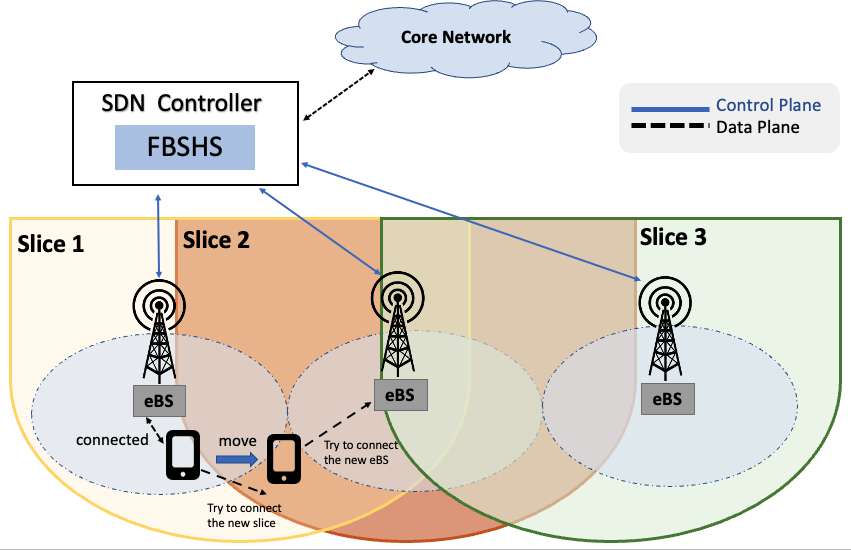
\includegraphics[width=1\textwidth]{figure/5GHO.png}
	\caption{Proposed system overview.}\label{fig:5GHO}
\end{figure}




%%%%%%%%%%%%%%%%%%%%%%%%%%%%%%%%%%%%%%%%%%%%%%%%%%%%%%%%%%%%%%%%%%%%%%%%%
%%%%%%%%%%%%%%%%%%%%%%%%%%%%%%%%%%%%%%%%%%%%%%%%%%%%%%%%%%%%%%%%%%%%%%%%%
%add image and title
\begin{figure}\centering
	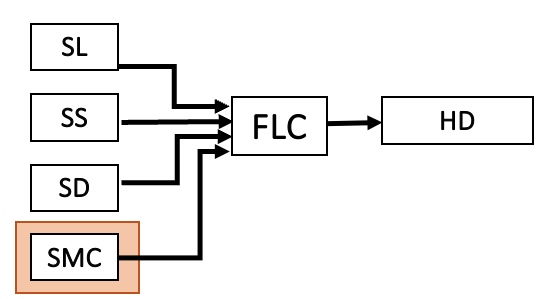
\includegraphics[width=0.65\textwidth]{figure/System/HODFLC.png}%imagine Avation
	\caption{Proposed system structure.}\label{fig:FLC1}
\end{figure}
%%%%%%%%%%%%%%%%%%%%%%%%%%%%%%%%%%%%%%%%%%%%%%%%%%%%%%%%%%%%%%%%%%%%%%%%%
%%%%%%%%%%%%%%%%%%%%%%%%%%%%%%%%%%%%%%%%%%%%%%%%%%%%%%%%%%%%%%%%%%%%%%%%%

 
In Fig.~\ref{fig:FLC1}, we show the proposed system structure. We describe in following the considered system parameters.

\textbf{Slice Load (SL):} When the SL increases, the slice becomes more congested, meaning that its resources are under heavy demand. This can lead to performance degradation and the system should make
HO to a less loaded slice.  Higher SL increases the HO probability because the load should be balanced 
to different slices.  

\textbf{Slice Stability (SS):} The SS refers to the capacity of a network slice to sustain consistent performance and QoS over the time, even during fluctuating network conditions or varying user demands. A NS with high stability guarantees reliable communication services and maintains steady performance, contributing to an enhanced user experience. On the other hand, if the SS is low, it indicates potential degradation in QoS. In such cases, the system initiates the HO to a more stable slice to ensure uninterrupted service and better performance.

\textbf{Slice Delay (SD):} The SD represents the latency experienced within a NS, typically resulting from data packet queuing and underlying network delays. A long SD can greatly affect the QoS. Such delays can lead to issues like lag, jitter, and disruptions, which are especially problematic for services that rely on immediate data transmission and low-latency performance.

\textbf{Slice Monetary Cost (SMC):} The SMC refers to the financial costs associated with deploying and maintaining NSs in 5G or B5G networks. Different slices might offer the same services at different costs due to variations in how resources are allocated, managed and optimized. The SMC can vary depending on the efficiency of the network infrastructure associated with each slice~\cite{walia2021virtualization}. The inter-slice HO possibility will be higher for slices with high monetary cost. 

\textbf{Handover Decision (HD):} The HD parameter is evaluated using the abovementioned four input parameters to determine whether to initiate or not the HO procedure. 

%%%%%%%%%%%%%%%%%%%%%%%%%%%%%%%%%%%%%%%%%%%%%%%%%%%%%%%%%%%%%%%%%%%%%%%%%
%%%%%%%%%%%%%%%%%%%%%%%%%%%%%%%%%%%%%%%%%%%%%%%%%%%%%%%%%%%%%%%%%%%%%%%%%
% Membership Table
%%%%%%%%%%%%%%%%%%%%%%%%%%%%%%%%%%%%%%%%%%%%%%%%%%%%%%%%%%%%%%%%%%%%%%%%%
%%%%%%%%%%%%%%%%%%%%%%%%%%%%%%%%%%%%%%%%%%%%%%%%%%%%%%%%%%%%%%%%%%%%%%%%%

%add table
\begin{table}\centering
	\caption{Parameter and their term sets.}
	\label{tab:Parameter}%\scriptsize
	\begin{tabular}{c | c }\hline
		Parameters & Term Sets \\\hline
	    Slice Load (SL) & Light Load(LL), Medium Load(ML), Heavy Load(HL) \\\hline
		Slice Stability (SS) & Unstable (Ue), Moderately Stable (MS), Stable (St) \\\hline
		Slice Delay (SD) & Very Low Delay (VLD), Low Delay (LD), Moderate Delay (MD), \\
		&High Delay (HD), Very High Delay (VHD) \\\hline
		Slice Monetary Cost (SMC) & Cheap (Cp), Moderate (Mt), Expensive (Ex) \\\hline 
		Handover Decision (HD) & ~HD1, HD2, HD3, HD4, HD5, \\
		& HD6, HD7, HD8, HD9\\
		\hline
	\end{tabular}	
\end{table}



\begin{table}\centering
	\caption{FRB.}
	\label{tab:rule base}%\scriptsize
		\scalebox{0.8}{
	\begin{tabular}{ |p{1cm}|p{1cm}|p{1cm}|p{1cm}|p{1cm}|p{1cm}|p{1cm}|p{1cm}|p{1cm}|p{1cm}|p{1cm}|p{1cm}|   }
	\hline
		Rule & SL & SS & SD & SMC & HD & Rule & SL & SS & SD & SMC & HD\\\hline
1	&	LL	&	Ue	&	VLD	&	Cp	&	HD1	&	68	&	ML	&	MS	&	MD	&	Mt	&	HD5	\\\hline
2	&	LL	&	Ue	&	VLD	&	Mt	&	HD2	&	69	&	ML	&	MS	&	MD	&	Ex	&	HD6	\\\hline
3	&	LL	&	Ue	&	VLD	&	Ex	&	HD3	&	70	&	ML	&	MS	&	HD	&	Cp	&	HD5	\\\hline
4	&	LL	&	Ue	&	LD	&	Cp	&	HD2	&	71	&	ML	&	MS	&	HD	&	Mt	&	HD6	\\\hline
5	&	LL	&	Ue	&	LD	&	Mt	&	HD3	&	72	&	ML	&	MS	&	HD	&	Ex	&	HD7	\\\hline
6	&	LL	&	Ue	&	LD	&	Ex	&	HD4	&	73	&	ML	&	MS	&	VHD	&	Cp	&	HD6	\\\hline
7	&	LL	&	Ue	&	MD	&	Cp	&	HD3	&	74	&	ML	&	MS	&	VHD	&	Mt	&	HD7	\\\hline
8	&	LL	&	Ue	&	MD	&	Mt	&	HD4	&	75	&	ML	&	MS	&	VHD	&	Ex	&	HD8	\\\hline
9	&	LL	&	Ue	&	MD	&	Ex	&	HD5	&	76	&	ML	&	St	&	VLD	&	Cp	&	HD1	\\\hline
10	&	LL	&	Ue	&	HD	&	Cp	&	HD4	&	77	&	ML	&	St	&	VLD	&	Mt	&	HD2	\\\hline
11	&	LL	&	Ue	&	HD	&	Mt	&	HD5	&	78	&	ML	&	St	&	VLD	&	Ex	&	HD3	\\\hline
12	&	LL	&	Ue	&	HD	&	Ex	&	HD6	&	79	&	ML	&	St	&	LD	&	Cp	&	HD1	\\\hline
13	&	LL	&	Ue	&	VHD	&	Cp	&	HD5	&	80	&	ML	&	St	&	LD	&	Mt	&	HD2	\\\hline
14	&	LL	&	Ue	&	VHD	&	Mt	&	HD6	&	81	&	ML	&	St	&	LD	&	Ex	&	HD3	\\\hline
15	&	LL	&	Ue	&	VHD	&	Ex	&	HD7	&	82	&	ML	&	St	&	MD	&	Cp	&	HD2	\\\hline
16	&	LL	&	MS	&	VLD	&	Cp	&	HD1	&	83	&	ML	&	St	&	MD	&	Mt	&	HD3	\\\hline
17	&	LL	&	MS	&	VLD	&	Mt	&	HD1	&	84	&	ML	&	St	&	MD	&	Ex	&	HD4	\\\hline
18	&	LL	&	MS	&	VLD	&	Ex	&	HD2	&	85	&	ML	&	St	&	HD	&	Cp	&	HD3	\\\hline
19	&	LL	&	MS	&	LD	&	Cp	&	HD1	&	86	&	ML	&	St	&	HD	&	Mt	&	HD4	\\\hline
20	&	LL	&	MS	&	LD	&	Mt	&	HD2	&	87	&	ML	&	St	&	HD	&	Ex	&	HD5	\\\hline
21	&	LL	&	MS	&	LD	&	Ex	&	HD3	&	88	&	ML	&	St	&	VHD	&	Cp	&	HD4	\\\hline
22	&	LL	&	MS	&	MD	&	Cp	&	HD2	&	89	&	ML	&	St	&	VHD	&	Mt	&	HD5	\\\hline
23	&	LL	&	MS	&	MD	&	Mt	&	HD3	&	90	&	ML	&	St	&	VHD	&	Ex	&	HD6	\\\hline
24	&	LL	&	MS	&	MD	&	Ex	&	HD4	&	91	&	HL	&	Ue	&	VLD	&	Cp	&	HD5	\\\hline
25	&	LL	&	MS	&	HD	&	Cp	&	HD3	&	92	&	HL	&	Ue	&	VLD	&	Mt	&	HD6	\\\hline
26	&	LL	&	MS	&	HD	&	Mt	&	HD4	&	93	&	HL	&	Ue	&	VLD	&	Ex	&	HD7	\\\hline
27	&	LL	&	MS	&	HD	&	Ex	&	HD5	&	94	&	HL	&	Ue	&	LD	&	Cp	&	HD6	\\\hline
28	&	LL	&	MS	&	VHD	&	Cp	&	HD4	&	95	&	HL	&	Ue	&	LD	&	Mt	&	HD7	\\\hline
29	&	LL	&	MS	&	VHD	&	Mt	&	HD5	&	96	&	HL	&	Ue	&	LD	&	Ex	&	HD8	\\\hline
30	&	LL	&	MS	&	VHD	&	Ex	&	HD6	&	97	&	HL	&	Ue	&	MD	&	Cp	&	HD7	\\\hline
31	&	LL	&	St	&	VLD	&	Cp	&	HD1	&	98	&	HL	&	Ue	&	MD	&	Mt	&	HD8	\\\hline
32	&	LL	&	St	&	VLD	&	Mt	&	HD1	&	99	&	HL	&	Ue	&	MD	&	Ex	&	HD9	\\\hline
33	&	LL	&	St	&	VLD	&	Ex	&	HD1	&	100	&	HL	&	Ue	&	HD	&	Cp	&	HD8	\\\hline
34	&	LL	&	St	&	LD	&	Cp	&	HD1	&	101	&	HL	&	Ue	&	HD	&	Mt	&	HD9	\\\hline
35	&	LL	&	St	&	LD	&	Mt	&	HD1	&	102	&	HL	&	Ue	&	HD	&	Ex	&	HD9	\\\hline
36	&	LL	&	St	&	LD	&	Ex	&	HD2	&	103	&	HL	&	Ue	&	VHD	&	Cp	&	HD9	\\\hline
37	&	LL	&	St	&	MD	&	Cp	&	HD1	&	104	&	HL	&	Ue	&	VHD	&	Mt	&	HD9	\\\hline
38	&	LL	&	St	&	MD	&	Mt	&	HD1	&	105	&	HL	&	Ue	&	VHD	&	Ex	&	HD9	\\\hline
39	&	LL	&	St	&	MD	&	Ex	&	HD2	&	106	&	HL	&	MS	&	VLD	&	Cp	&	HD4	\\\hline
40	&	LL	&	St	&	HD	&	Cp	&	HD1	&	107	&	HL	&	MS	&	VLD	&	Mt	&	HD5	\\\hline
41	&	LL	&	St	&	HD	&	Mt	&	HD2	&	108	&	HL	&	MS	&	VLD	&	Ex	&	HD6	\\\hline
42	&	LL	&	St	&	HD	&	Ex	&	HD3	&	109	&	HL	&	MS	&	LD	&	Cp	&	HD5	\\\hline
43	&	LL	&	St	&	VHD	&	Cp	&	HD2	&	110	&	HL	&	MS	&	LD	&	Mt	&	HD6	\\\hline
44	&	LL	&	St	&	VHD	&	Mt	&	HD3	&	111	&	HL	&	MS	&	LD	&	Ex	&	HD7	\\\hline
45	&	LL	&	St	&	VHD	&	Ex	&	HD4	&	112	&	HL	&	MS	&	MD	&	Cp	&	HD6	\\\hline
46	&	ML	&	Ue	&	VLD	&	Cp	&	HD3	&	113	&	HL	&	MS	&	MD	&	Mt	&	HD7	\\\hline
47	&	ML	&	Ue	&	VLD	&	Mt	&	HD4	&	114	&	HL	&	MS	&	MD	&	Ex	&	HD8	\\\hline
48	&	ML	&	Ue	&	VLD	&	Ex	&	HD5	&	115	&	HL	&	MS	&	HD	&	Cp	&	HD7	\\\hline
49	&	ML	&	Ue	&	LD	&	Cp	&	HD4	&	116	&	HL	&	MS	&	HD	&	Mt	&	HD8	\\\hline
50	&	ML	&	Ue	&	LD	&	Mt	&	HD5	&	117	&	HL	&	MS	&	HD	&	Ex	&	HD9	\\\hline
51	&	ML	&	Ue	&	LD	&	Ex	&	HD6	&	118	&	HL	&	MS	&	VHD	&	Cp	&	HD8	\\\hline
52	&	ML	&	Ue	&	MD	&	Cp	&	HD5	&	119	&	HL	&	MS	&	VHD	&	Mt	&	HD9	\\\hline
53	&	ML	&	Ue	&	MD	&	Mt	&	HD6	&	120	&	HL	&	MS	&	VHD	&	Ex	&	HD9	\\\hline
54	&	ML	&	Ue	&	MD	&	Ex	&	HD7	&	121	&	HL	&	St	&	VLD	&	Cp	&	HD2	\\\hline
55	&	ML	&	Ue	&	HD	&	Cp	&	HD6	&	122	&	HL	&	St	&	VLD	&	Mt	&	HD3	\\\hline
56	&	ML	&	Ue	&	HD	&	Mt	&	HD7	&	123	&	HL	&	St	&	VLD	&	Ex	&	HD4	\\\hline
57	&	ML	&	Ue	&	HD	&	Ex	&	HD8	&	124	&	HL	&	St	&	LD	&	Cp	&	HD3	\\\hline
58	&	ML	&	Ue	&	VHD	&	Cp	&	HD7	&	125	&	HL	&	St	&	LD	&	Mt	&	HD4	\\\hline
59	&	ML	&	Ue	&	VHD	&	Mt	&	HD8	&	126	&	HL	&	St	&	LD	&	Ex	&	HD5	\\\hline
60	&	ML	&	Ue	&	VHD	&	Ex	&	HD9	&	127	&	HL	&	St	&	MD	&	Cp	&	HD4	\\\hline
61	&	ML	&	MS	&	VLD	&	Cp	&	HD2	&	128	&	HL	&	St	&	MD	&	Mt	&	HD5	\\\hline
62	&	ML	&	MS	&	VLD	&	Mt	&	HD3	&	129	&	HL	&	St	&	MD	&	Ex	&	HD6	\\\hline
63	&	ML	&	MS	&	VLD	&	Ex	&	HD4	&	130	&	HL	&	St	&	HD	&	Cp	&	HD5	\\\hline
64	&	ML	&	MS	&	LD	&	Cp	&	HD3	&	131	&	HL	&	St	&	HD	&	Mt	&	HD6	\\\hline
65	&	ML	&	MS	&	LD	&	Mt	&	HD4	&	132	&	HL	&	St	&	HD	&	Ex	&	HD7	\\\hline
66	&	ML	&	MS	&	LD	&	Ex	&	HD5	&	133	&	HL	&	St	&	VHD	&	Cp	&	HD6	\\\hline
67	&	ML	&	MS	&	MD	&	Cp	&	HD4	&	134	&	HL	&	St	&	VHD	&	Mt	&	HD7	\\\hline
	&		&		&		&		&		&	135	&	HL	&	St	&	VHD	&	Ex	&	HD8	\\\hline
		
	\end{tabular}}
\end{table}			
%%%%%%%%%%%%%%%%%%%%%%%%%%%%%%%%%%%%%%%%%%%%%%%%%%%%%%%%%%%%%%%%%%%%%%%%%
%%%%%%%%%%%%%%%%%%%%%%%%%%%%%%%%%%%%%%%%%%%%%%%%%%%%%%%%%%%%%%%%%%%%%%%%%
% Membership functions
%%%%%%%%%%%%%%%%%%%%%%%%%%%%%%%%%%%%%%%%%%%%%%%%%%%%%%%%%%%%%%%%%%%%%%%%%
%%%%%%%%%%%%%%%%%%%%%%%%%%%%%%%%%%%%%%%%%%%%%%%%%%%%%%%%%%%%%%%%%%%%%%%%%
%Membership function
%\vspace{20mm}
\begin{figure*}\centering
	\subfigure[Slice Load]{
		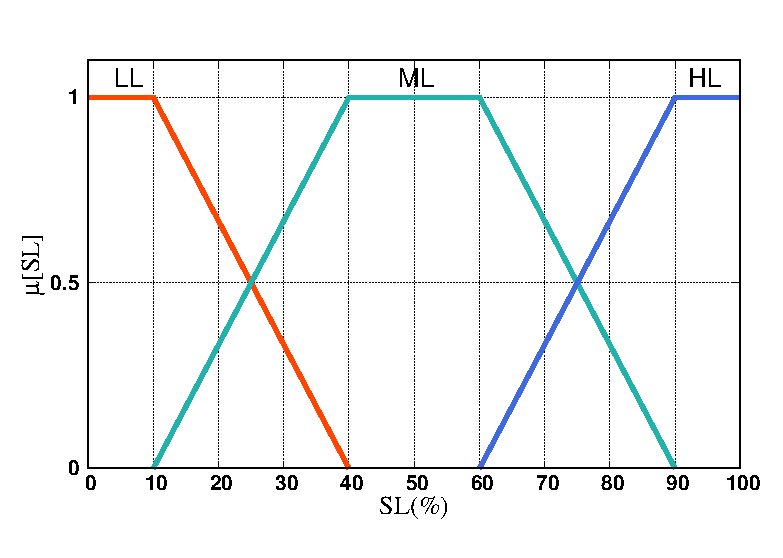
\includegraphics[width=0.48\textwidth]{figure/Membership/SL.eps}
		\label{subfig:MB1}
	}
	\subfigure[Slice Stability]{
		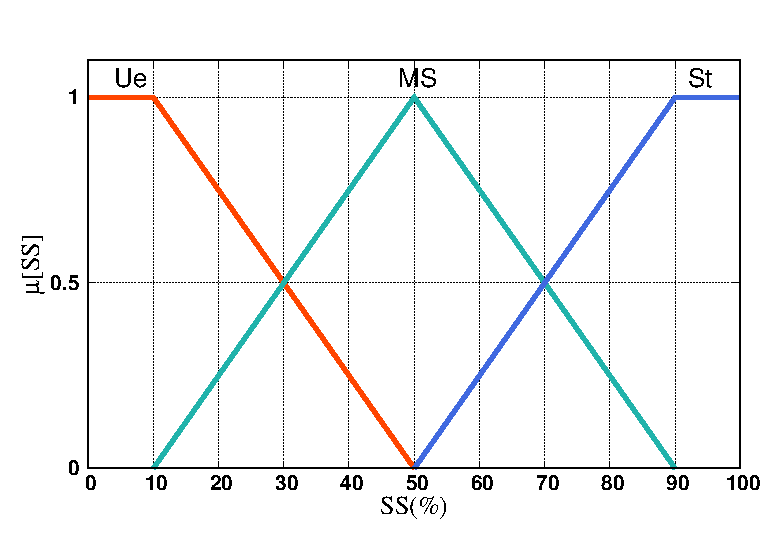
\includegraphics[width=0.48\textwidth]{figure/Membership/SS.eps}
		\label{subfig:MB2}
	}
	\subfigure[Slice Delay]{
		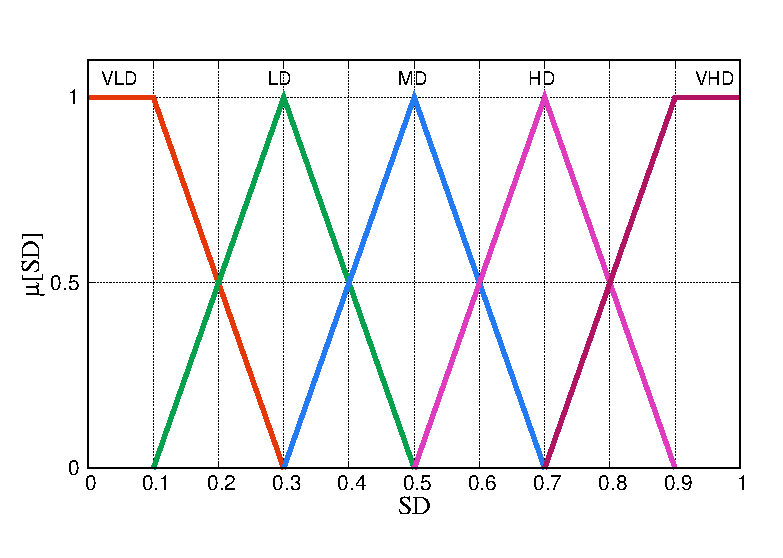
\includegraphics[width=0.48\textwidth]{figure/Membership/SD.eps}
		\label{subfig:MB3}
	}
		\subfigure[Slice Monetary Cost]{
		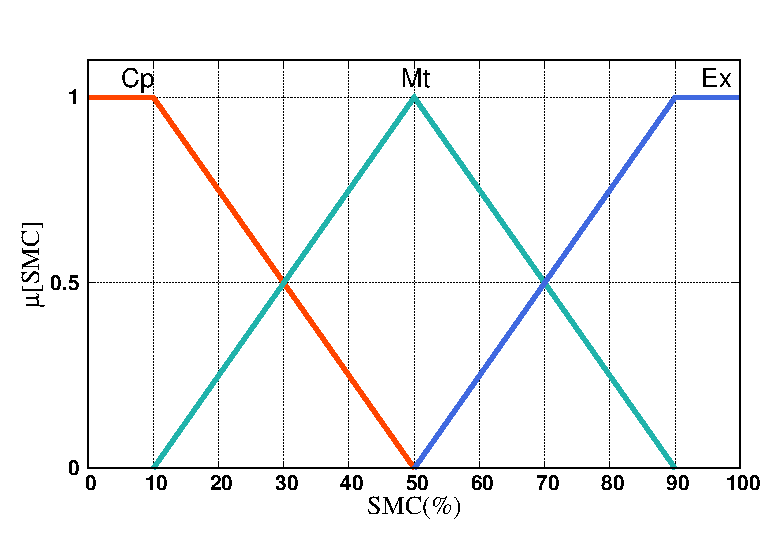
\includegraphics[width=0.48\textwidth]{figure/Membership/SMC.eps}
		\label{subfig:MB4}
	}
	\subfigure[Handover Decision]{
		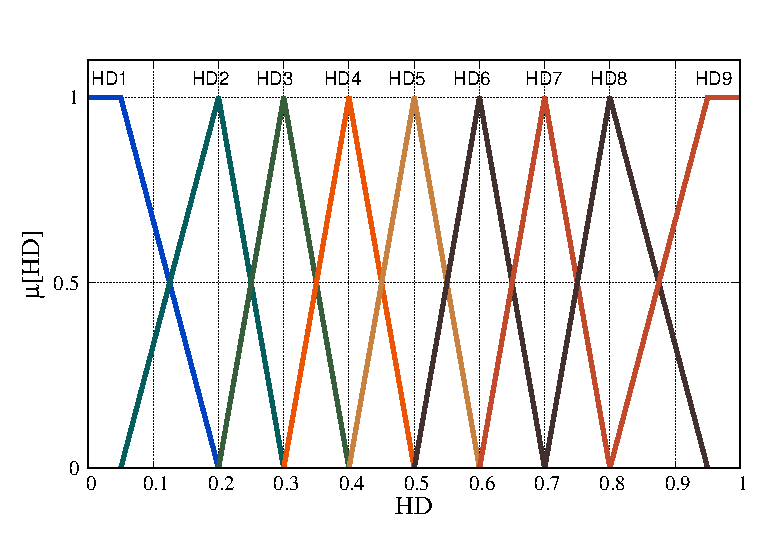
\includegraphics[width=0.48\textwidth]{figure/Membership/HD9.eps}
		\label{subfig:MB5}
	}
	\caption{\label{fig:MB}Membership functions.}
\end{figure*}

In Table \ref{tab:Parameter}, we present both the input parameters (SL, SS, SD, SMC) and the output parameter (HD) along with their associated term sets. While in Fig.~\ref{fig:MB}, we show the memership functions. For instance, SL is categorized as Light Load, Medium Load or Heavy Load, while SS is classified as Unstable, Moderately Stable or Stable. The output parameter (HD), is divided into seven levels, ranging from HD1 to HD7. To enable real-time operation, we utilize triangular and trapezoidal membership functions due to their simplicity and computational efficiency. The Fuzzy Rule Base (FRB) is developed using a set of 135 rules structured as "IF [condition] THEN [control action]". This comprehensive rule base allows the system to assess various combinations of input parameters and adaptively make HD decision.

%%%%%%%%%%%%%%%%%%%%%%%%%%%%%%%%%%%%%%%%%%%%%%%%%%%%%%%%%%%%%%%%%%%%%%%%%
%%%%%%%%%%%%%%%%%%%%%%%%%%%%%%%%%%%%%%%%%%%%%%%%%%%%%%%%%%%%%%%%%%%%%%%%%
%Simulation Results
%%%%%%%%%%%%%%%%%%%%%%%%%%%%%%%%%%%%%%%%%%%%%%%%%%%%%%%%%%%%%%%%%%%%%%%%%
%%%%%%%%%%%%%%%%%%%%%%%%%%%%%%%%%%%%%%%%%%%%%%%%%%%%%%%%%%%%%%%%%%%%%%%%%
 
%\vspace{100mm}
\section{Simulation Results}\label{sec:sim-results}
We present the simulation results of our proposed system in Fig.~\ref{fig:SLL}, Fig.~\ref{fig:SLM}, and Fig.~\ref{fig:SLH} for different SL values 10\%, 50\%, and 90\%, respectively. The output parameter, denoted as HD, is analyzed in relation to four input parameters: SL, SS, SD, and SMC. 

 
 %%%%% SL - 10% %%%%%%%%
In Fig.~\ref{fig:SLL}~(a), SL value is 10\% and SS value is 10\%. For SD 90\%, we changed the SMC values from 10\% to 50\% and from 50\% to 90\%. We observed that the HD values increased by 10\% in both cases. Considering other SD values less than 50\%, the HD value is less than 0.5. This means that for small SL, moderate SD, and small SS, the HO process will not be carried out. However, when the serving slice has a very high delay, unstable service, and higher cost, the inter-slice handover is needed. In Fig.~\ref{fig:SLL}~(b), the SS value is increasing to 90\%, which shows that the serving slice is more stable than Fig.~\ref{fig:SLL}~(a). All HD values are below 0.5, indicating that the likelihood of a HO is low regardless of the values of other parameters.

 %%%%% SL - 50% %%%%%%%%
For SS 10\%, we increased the SL value from 10\% to 50\% (see Fig.~\ref{fig:SLL}~(a)) and then
to 90\% (see Fig.~\ref{fig:SLM}~(a)). In these cases, when SD is 70\% and SMC is 50\%, the HD is increasing by 20\%. In Fig.~\ref{fig:SLM}~(a), we see that when the SD values increase from 10\% to 90\%, the HD values also increase. When the SMC value is 50\% and for SD more than 50\%, all  HD values are higher than 0.5. This means that for these cases the HO procees is needed. Comparing Fig.~\ref{fig:SLM}~(b) with Fig.~\ref{fig:SLL}~(b), we see that the increase of SL increases the HO possibility. 
  
 %%%%% SL - 90% %%%%%%%%
When the SL value is increased to 90\% in Fig.~\ref{fig:SLH}~(a) and SS value is 10\%, the HD values are significantly higher compared with other scenarios. All HD values are higher than 0.5. This is because the serving slice has a heavy load and an unstable service resulting in inter-slice HO. However, when the SS value is increased from 10\% to 90\%, the HD values are decreasing. For SMC values below 50\% and SD values ranging from 10\% to 50\%, the HD values are below 0.5. Thus, the HO process is not needed.
   

%%%%%%%%%%%%%%%%%%%%%%%%%%%%%%%%%%%%%%%%%%%%%%%%%%%%%%%%%%%%%%%%%%%%%%%%%
%%%%%%%%%%%%%%%%%%%%%%%%%%%%%%%%%%%%%%%%%%%%%%%%%%%%%%%%%%%%%%%%%%%%%%%%%

%%%%%%%%%%%%%%%%%%%%%%%%%%%%%%%%%%%%%%%%%%%%%%%%%%%%%%%%%%%%%%%%%%%%%%%%%
%. result img
%%%%%%%%%%%%%%%%%%%%%%%%%%%%%%%%%%%%%%%%%%%%%%%%%%%%%%%%%%%%%%%%%%%%%%%%%
\begin{figure*}\centering
    \subfigure[SS=10\%]{
        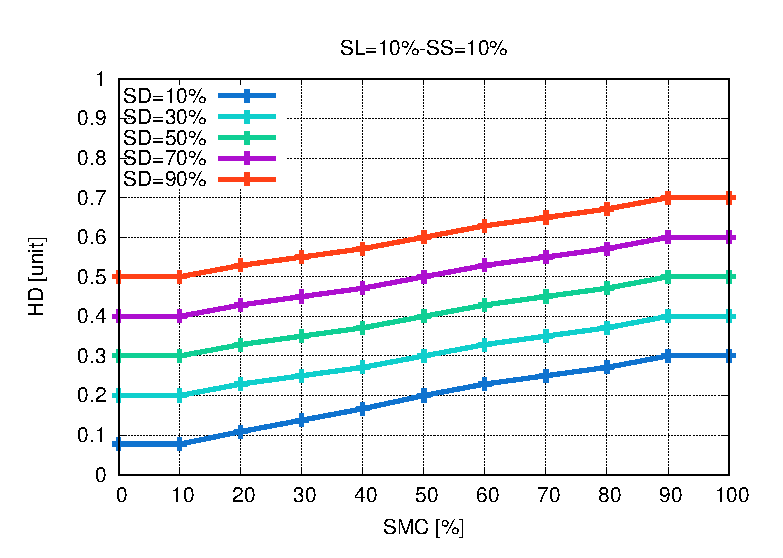
\includegraphics[width=0.45\textwidth]{figure/results/SL=0.1-SS=0.1.eps}
        \label{subfig:SS1}
    }
%    \subfigure[SS=50\%]{
%        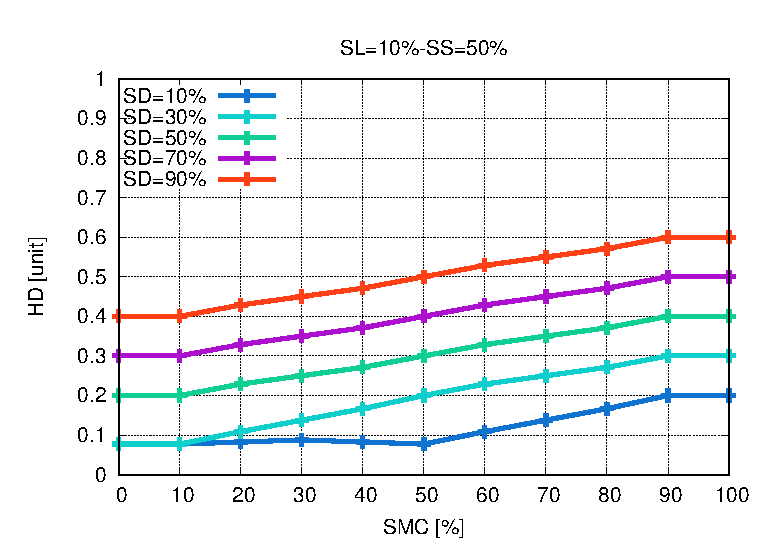
\includegraphics[width=0.45\textwidth]{figure/results/SL=0.1-SS=0.5.eps}
%        \label{subfig:SS2}
%    }
    \subfigure[SS=90\%]{
        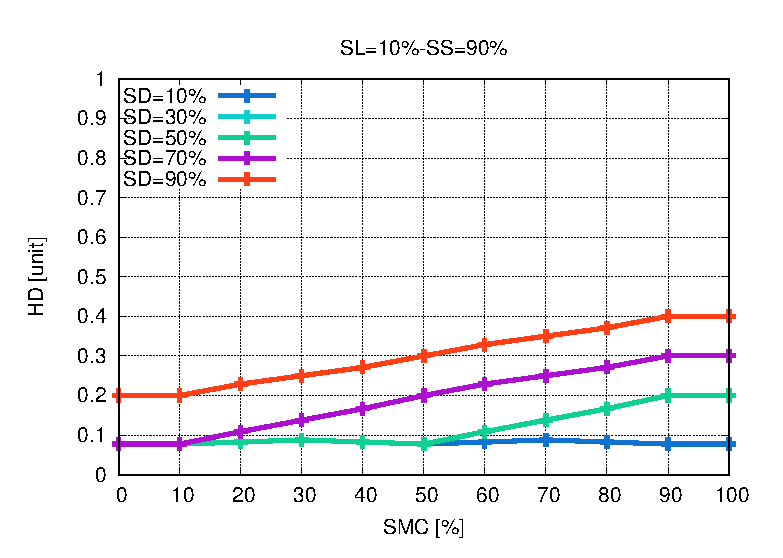
\includegraphics[width=0.45\textwidth]{figure/results/SL=0.1-SS=0.9.eps}
        \label{subfig:SS3}
    }
    \caption{\label{fig:SLL}Simulation results for SL=10\%.}
\end{figure*}


\begin{figure*}\centering
    \subfigure[SS=10\%]{
        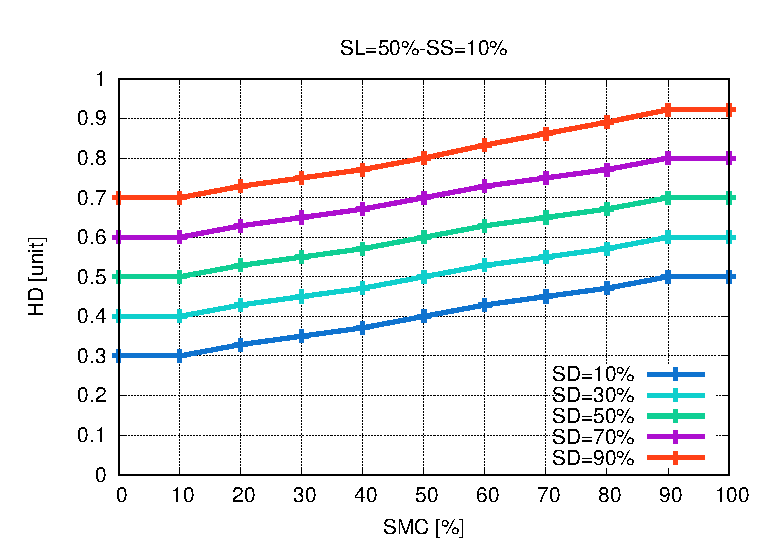
\includegraphics[width=0.45\textwidth]{figure/results/SL=0.5-SS=0.1.eps}
        \label{subfig:SS4}
    }
%    \subfigure[SS=50\%]{
%        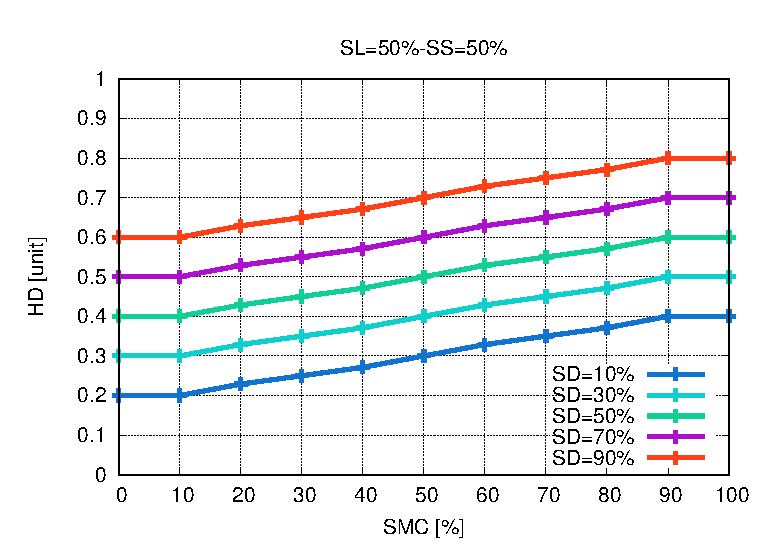
\includegraphics[width=0.45\textwidth]{figure/results/SL=0.5-SS=0.5.eps}
%        \label{subfig:SS5}
%    }
    \subfigure[SS=90\%]{
        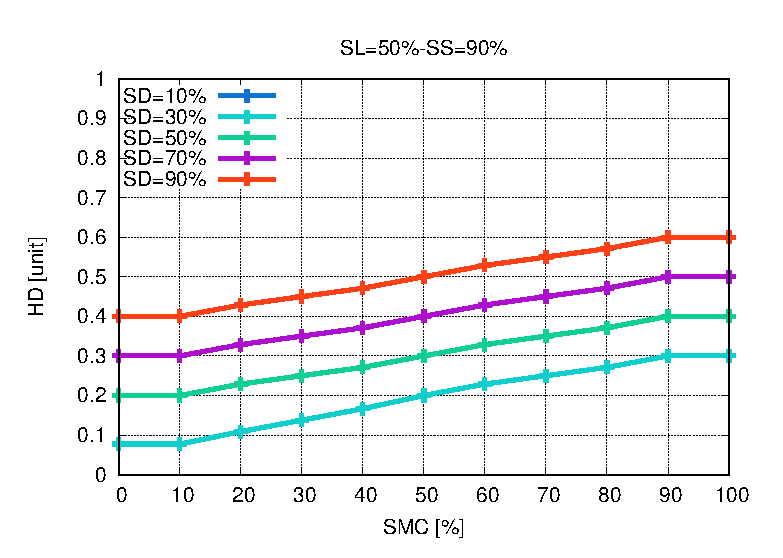
\includegraphics[width=0.45\textwidth]{figure/results/SL=0.5-SS=0.9.eps}
        \label{subfig:SS6}
    }
    \caption{\label{fig:SLM}Simulation results for SL=50\%.}
\end{figure*}


\begin{figure*}\centering
    \subfigure[SS=10\%]{
        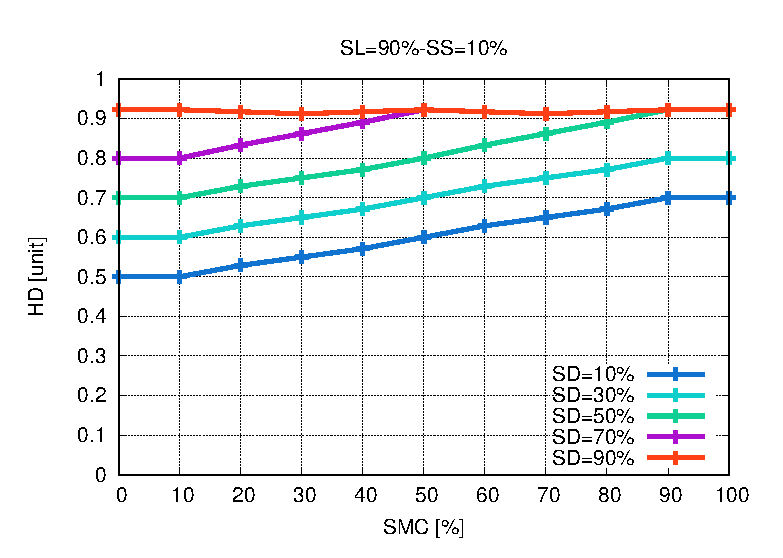
\includegraphics[width=0.45\textwidth]{figure/results/SL=0.9-SS=0.1.eps}
        \label{subfig:SS4}
    }
%    \subfigure[SS=50\%]{
%        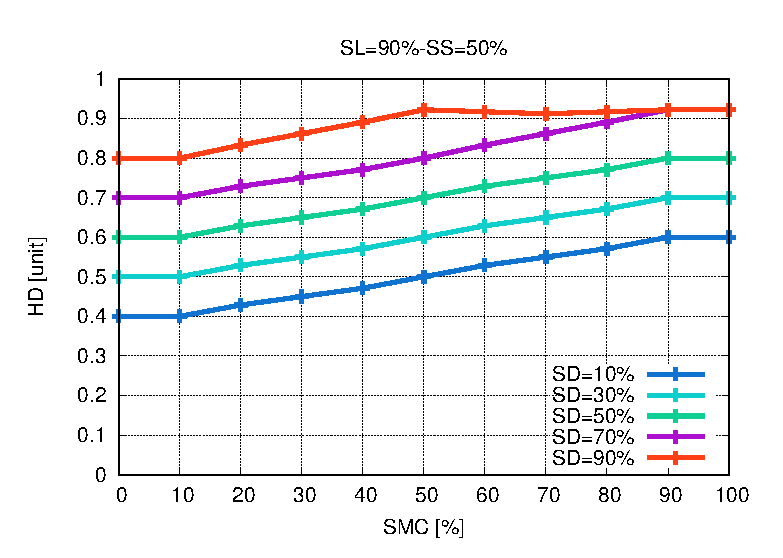
\includegraphics[width=0.45\textwidth]{figure/results/SL=0.9-SS=0.5.eps}
%        \label{subfig:RS5}
%    }
    \subfigure[SS=90\%]{
        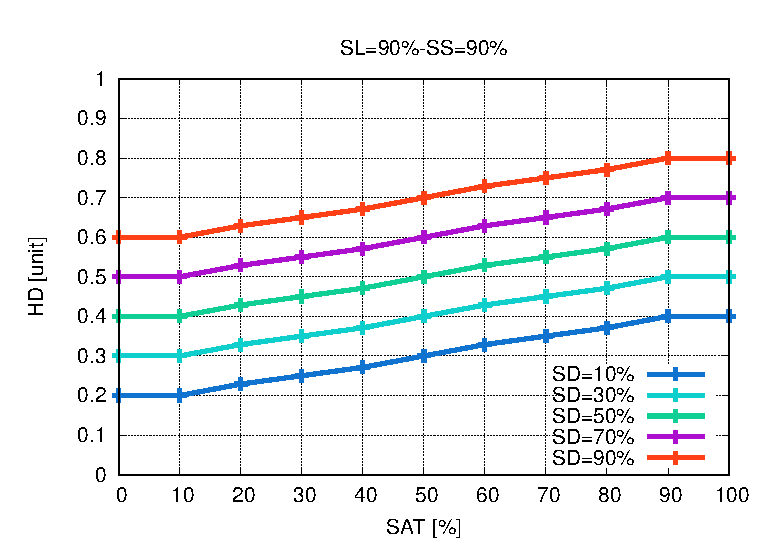
\includegraphics[width=0.45\textwidth]{figure/results/SL=0.9-SS=0.9.eps}
        \label{subfig:SS6}
    }
    \caption{\label{fig:SLH}Simulation results for SL=90\%.}
\end{figure*}



%%%%%%%%%%%%%%%%%%%%%%%%%%%%%%%%%%%%%%%%%%%%%%%%%%%%%%%%%%%%%%%%%%%%%%%%%
%%%%%%%%%%%%%%%%%%%%%%%%%%%%%%%%%%%%%%%%%%%%%%%%%%%%%%%%%%%%%%%%%%%%%%%%%
% Conclusions and Future Work
%%%%%%%%%%%%%%%%%%%%%%%%%%%%%%%%%%%%%%%%%%%%%%%%%%%%%%%%%%%%%%%%%%%%%%%%%
%%%%%%%%%%%%%%%%%%%%%%%%%%%%%%%%%%%%%%%%%%%%%%%%%%%%%%%%%%%%%%%%%%%%%%%%%
\section{Conclusions and Future Work}\label{sec:conclusions}

In this paper, we proposed a Fuzzy-based HO system for 5G/B5G wireless networks considering four parameters: SL, SS, SD and SMC, which is a new parameter. The simulation results indicate that these parameters have different effects on the HD. When SL, SD and SMC increase, the probability of the HD is increased. However, the SS reduces the HD probability and the user remains in the serving slice.

In future work, we plan to incorporate additional parameters and perform comprehensive simulations to assess the effectiveness of the proposed system.

%%%%%%%%%%%%%%%%%%%%%%%%%%%%%%%%%%%%%%%%%%%%%%%%%%%%%%%%%%%%%%%%%%%%%%%%%
%%%%%%%%%%%%%%%%%%%%%%%%%%%%%%%%%%%%%%%%%%%%%%%%%%%%%%%%%%%%%%%%%%%%%%%%%


%\vspace{350cm}
%\begin{thebibliography}{10}
%\bibitem{Akyildiz}  
%Akyildiz  F.I., Wang X., Wang W.: Wireless Mesh Networks: A
%Survey. In: Computer Networks, Vol. 47, No. 4, pp. 445-487, 2005.

%\bibliographystyle{IEEEtran}
%\bibliographystyle{junsrt}		%出てきた順索引 
%\bibliographystyle{spbasic}
%\bibliographystyle{splncs04}
%\bibliographystyle{ieeetr}
\bibliographystyle{spmpsci}
%\bibliographystyle{splncs}

\bibliography{Ref}

\end{document}
